\begin{table}[]
    \centering
    \caption[Algorithmic characterization of embedding operations.]{Algorithmic characterization of the embedding operations studied in \Cref{sec:embedding-workload-characterization}. The table summarizes each operation's loop hierarchy and its compute-per-lookup ratio, using one dense embedding-vector lookup as the normalization baseline. The ratio counts vector arithmetic operations performed for each irregular vector lookup. EB performs one vector accumulation per lookup, KGs perform four vector operations across three lookups, SpMM performs one rescale and one accumulation per lookup, and MP reaches the highest ratio with at most five vector operations across two lookups. SpAttn performs no arithmetic on the looked-up vectors in this characterization because it copies sparse-attention blocks. Thus, the compute-per-lookup ratio ranges from 0 to at most 2.5, showing that these embedding operations expose little arithmetic work per irregular lookup and therefore give compute-oriented architectures limited opportunity to hide lookup latency.}
    \begin{tabular}{clc}
        \toprule
            \makecell[c]{\textbf{Op}} & 
            \makecell[l]{\textbf{Loop hierarchy}} & 
            $\frac{\textbf{N}_\textbf{compute}}{\textbf{N}_\textbf{lookups}}$\\
        \toprule
            \makecell[c]{SpMM \\(GNNs)} &% \\ (\Cref{sec:embedding-characterization-graph-learning})} &
            \makecell[l]{$\forall$ vertex in graph\\
                        \hspace{0.5em}$\forall$ neighbor of vertex\\
                            \hspace{1em}\textbf{lookup} vector\\
                            \hspace{1em}\textbf{rescale} vector\\
                            \hspace{1em}\textbf{accumulate} vector} &
            $\frac{2}{1}$\\
        \hline
            \makecell[c]{MP} &% \\ (\Cref{sec:embedding-characterization-graph-learning})} &
            \makecell[l]{$\forall$ vertex in graph\\
                        \hspace{0.5em}\textbf{lookup} vertex vector\\
                        \hspace{0.5em}$\forall$ neighbor of vertex\\
                            \hspace{1em}\textbf{lookup} neighbor vector\\
                            \hspace{1em}\textbf{multiply} vert-neigh vecs\\
                            \hspace{1em}\textbf{scale} and \textbf{accumulate} vec\\
                        \hspace{0.5em}\textbf{multiply-accumulate} vec} &
            $\leq\frac{5}{2}$\\
        \hline
            \makecell[c]{KGs} &% \\ (\Cref{sec:embedding-characterization-graph-learning})} &
            \makecell[l]{$\forall$ sample in batch\\
                            \hspace{0.5em}\textbf{lookup} vector\\
                            \hspace{0.5em}\textbf{compute} h-r-l norm} &
            $\frac{4}{3}$\\
        \hline
            \makecell[c]{EB \\ (DLRMs)} &% \\ (\Cref{sec:embedding-characterization-dlrms})} &
            \makecell[l]{$\forall$ segment in batch\\
                            \hspace{0.5em}$\forall$ category in segment\\
                                \hspace{1.0em}\textbf{lookup} vector\\
                                \hspace{1.0em}\textbf{accumulate} vector} &
            $\frac{1}{1}$\\
        \hline
            \makecell[c]{SpAttn \\ (LLMs)} &% \\ (\Cref{sec:embedding-characterization-llms})} &
            \makecell[l]{$\forall$ block in Q input\\
                        \hspace{0.5em}$\forall$ block in K input\\
                            \hspace{1.0em}$\forall$ token in K block\\
                                \hspace{1.5em}\textbf{lookup} K vector\\
                                \hspace{1.5em}$\forall$ token in Q block\\
                                    \hspace{2em}\textbf{copy} K vector} &
            $0$\\
        \bottomrule
    \end{tabular}
    \label{tab:embedding-workload-code-characterization}
\end{table}

\begin{table}[]
    \centering
    \caption[Memory characterization of embedding operations.]{Memory characterization of the embedding operations studied in \Cref{sec:embedding-workload-characterization}. The table reports embedding storage requirements, temporal locality, and spatial locality. Temporal locality is measured with the reuse-distance CDF: the x-axis is cache capacity measured in embedding vectors, and the y-axis is the fraction of accesses whose reuse distance is below that capacity. Thus, the y-value approximates the hit probability of a cache that can hold the corresponding number of embedding vectors. Spatial locality is measured by the number of elements fetched per embedding-vector lookup. Temporal locality varies widely across workloads and inputs. At a reuse distance of 1K vectors, GNN CDFs stay below 20\%---meaning that fewer than 20\% of accesses have reuse distance below 1K vectors---and KGs below 10\%, while MP ranges from below 5\% to roughly 45\% depending on the input graph. DLRMs exhibit higher but feature-dependent locality, with Criteo features reaching about 63\%--99\% CDF at 1K vectors. Sparse attention locality depends strongly on block size: larger blocks increase the CDF but also increase copied-vector work. Spatial locality also varies widely, from 8--349 elements for GNNs, 128 for MP, 512 for KGs, 32--256 for EB, and up to $8\times8\times512$ elements for sparse attention blocks. Together, these ranges show that embedding workloads need architectures that adapt to widely different temporal and spatial locality regimes, exploiting cache reuse when it exists while also sustaining low-reuse vector lookups with different vector sizes.}
    \begin{tabular}{ccccc}
        \toprule
            \makecell[c]{\textbf{Op}} & 
            \makecell[c]{\textbf{Memory} \\ \textbf{footprint}} &
            \makecell[c]{\textbf{Temporal locality} \\ \textbf{(reuse distance CDF)}} &
            \makecell[c]{\textbf{Spatial locality} \\ \textbf{(vector dim.)}}\\
        \toprule
            \makecell[c]{SpMM \\(GNNs)} &% \\ (\Cref{sec:embedding-characterization-graph-learning})} &
            \makecell{Single embedding \\ table GBs large} &
            \vcentered{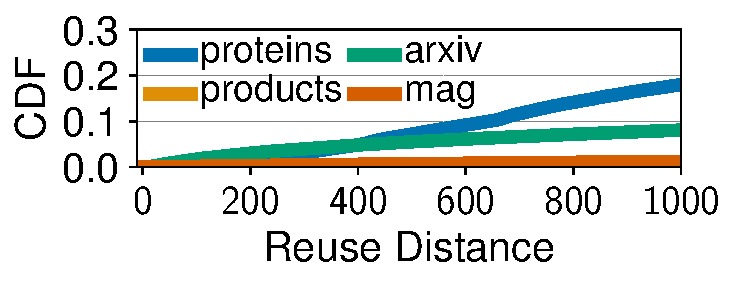
\includegraphics[width=.35\linewidth]{img_cdf_gnn.pdf}} &
            8-349\\ 
        \hline
            \makecell[c]{MP} &% \\ (\Cref{sec:embedding-characterization-graph-learning})} &
            \makecell{Two embedding tables, \\ each GBs large} &
            \vcentered{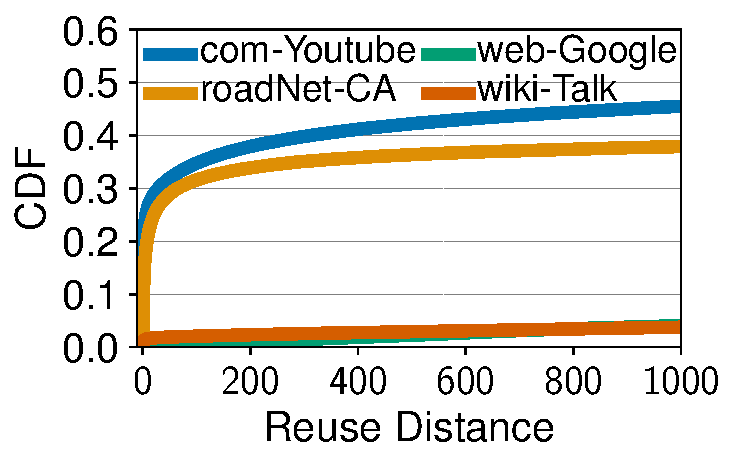
\includegraphics[width=.35\linewidth]{img_cdf_mp.pdf}} &
            128\\
        \hline
            \makecell[c]{KGs} &% \\ (\Cref{sec:embedding-characterization-graph-learning})} &
            \makecell{Single embedding \\ table GBs large} &
            \vcentered{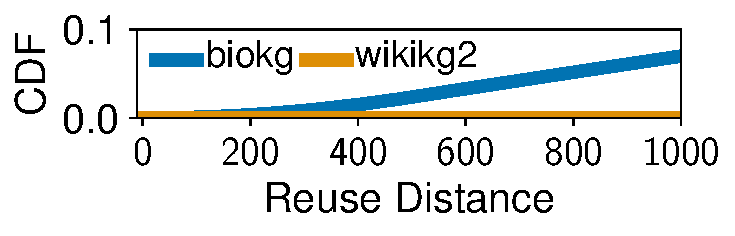
\includegraphics[width=.35\linewidth]{img_cdf_kg.pdf}} &
            512\\
        \hline
            \makecell[c]{EB \\ (DLRMs)} &% \\ (\Cref{sec:embedding-characterization-dlrms})} &
            \makecell{All embedding tables \\ require GBs~\cite{gupta2020hpca}\\ to TBs~\cite{ibrahim2022memsys}} &
            \vcentered{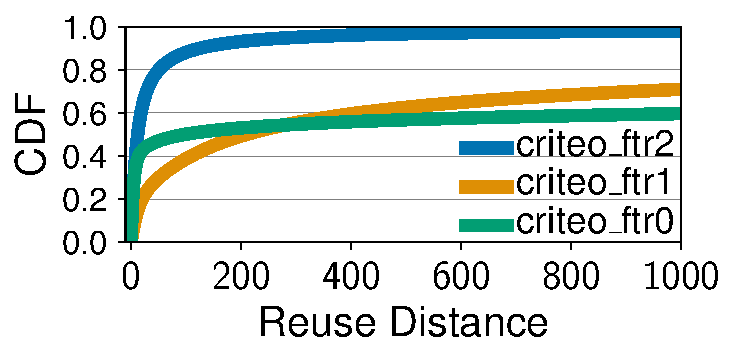
\includegraphics[width=.35\linewidth]{img_cdf_dlrm.pdf}} &
            32-256\\
        \hline
            \makecell[c]{SpAttn \\ (LLMs)} &% \\ (\Cref{sec:embedding-characterization-llms})} &
            \makecell{K-V tensors are MBs \\ Out tensor is MB-GB} &
            \vcentered{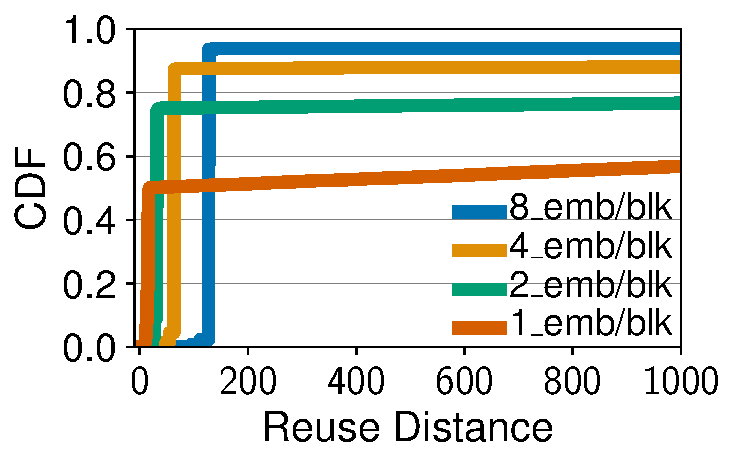
\includegraphics[width=.35\linewidth]{img_cdf_llm.pdf}} &
            $\leq$ 8x8x512\\
        \bottomrule
    \end{tabular}
    \label{tab:embedding-workload-locality-characterization}
\end{table}
